\documentclass[
	%parspace, % Add vertical space between paragraphs
	%noindent, % No indentation of first lines in each paragraph
	%nohyp, % No hyphenation of words
	%twoside, % Double sided format
	%draft, % Quicker draft compilation without rendering images
	%final, % Set final to hide todos
]{elteikthesis}[2024/04/26]

% Document's metadata
\title{Nagy nyelvi modellek mint kód olvashatósági elemzők}
\date{2026}

% Author's metadata
\author{Márton Gergő}
\degree{programtervező informatikus MSc}

% Superivsor(s)' metadata
\supervisor{Szalontai Balázs}
\affiliation{egyetemi tanársegéd}

% University's metadata
\university{Eötvös Loránd Tudományegyetem}
\faculty{Informatikai Kar}
\department{Programozáselméleti és Szoftvertechnológiai Tanszék}
\city{Budapest}
\logo{elte_cimer_szines}

% Add bibliography file
\addbibresource{diplomamunka.bib}

% The document
\begin{document}
\documentlang{hungarian}

% Title page (mandatory)
\maketitle

% Topic declaration page (mandatory) - can also be attached instead
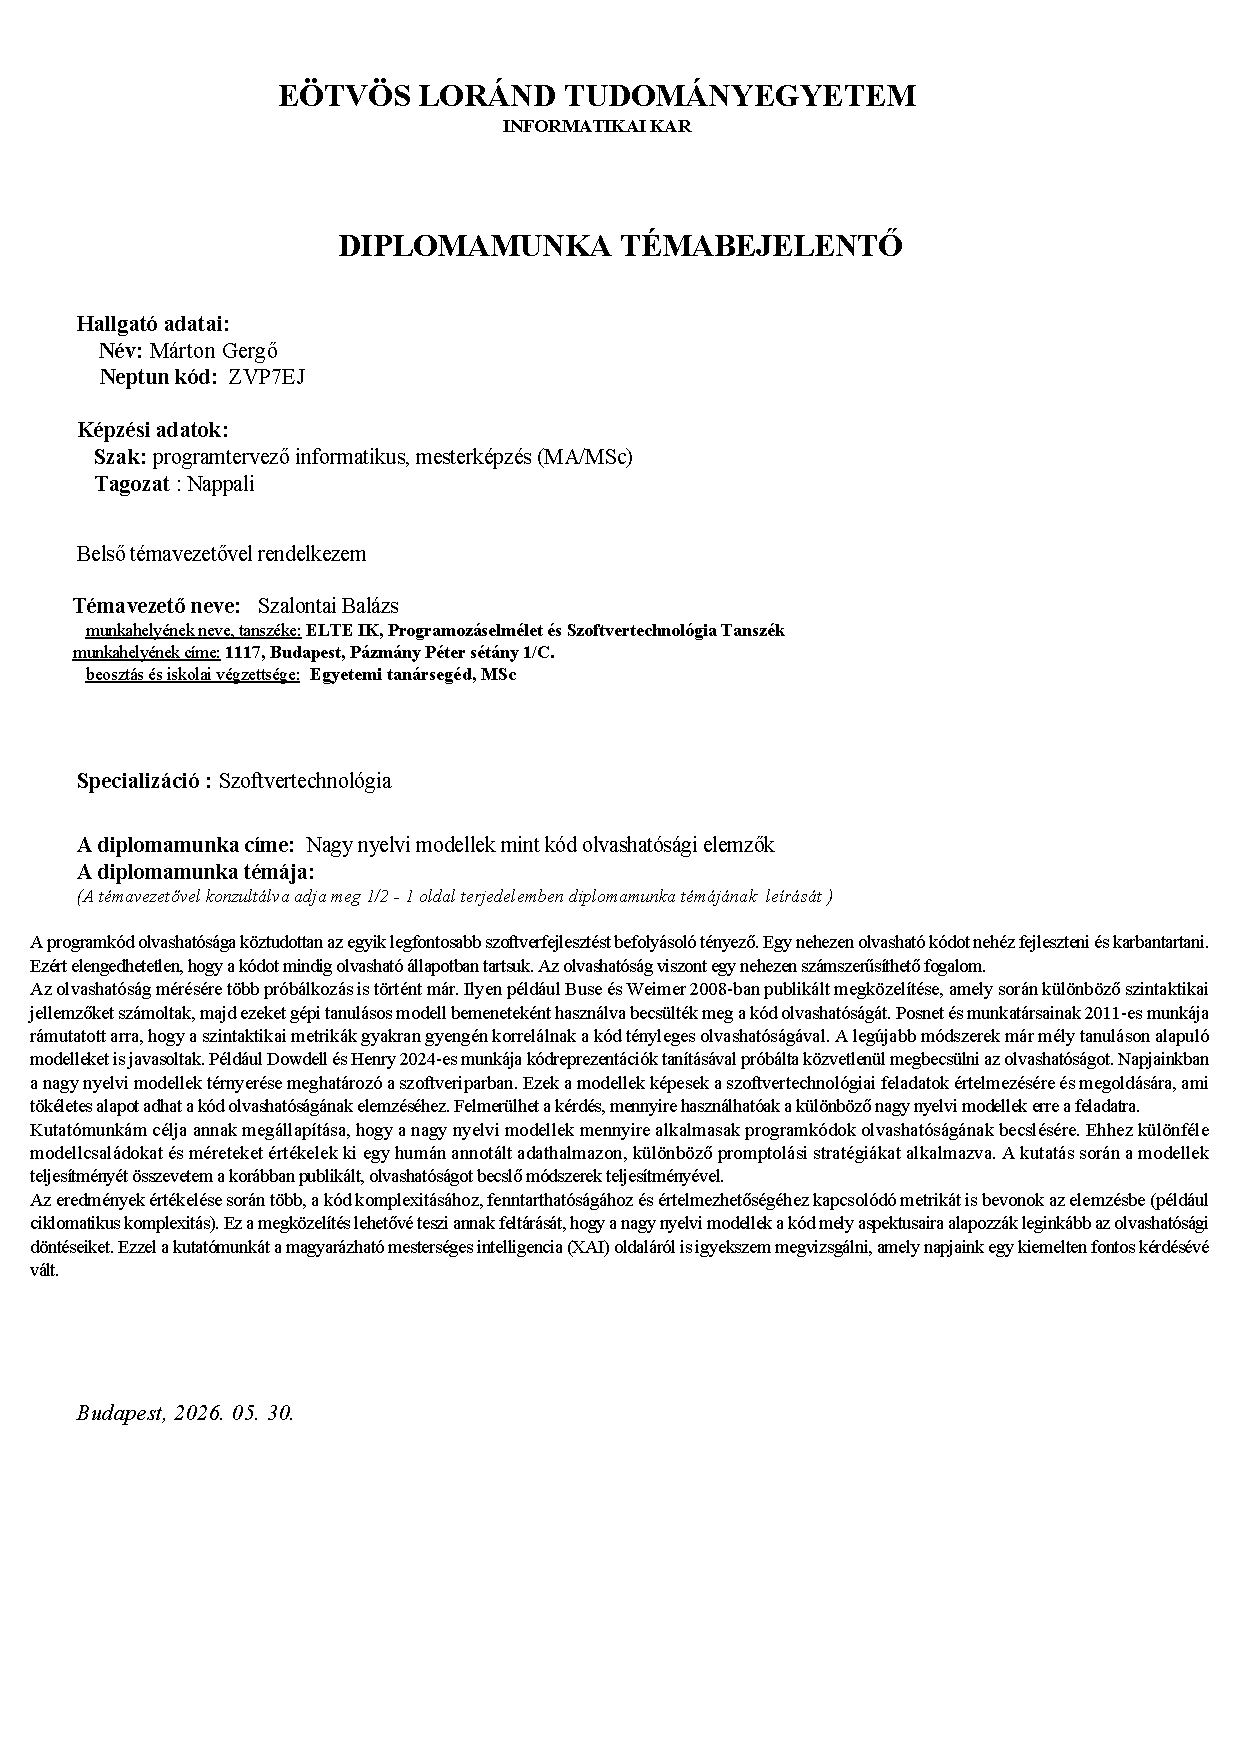
\includepdf{temabejelento.pdf}

% Table of contents (mandatory)
\tableofcontents
\cleardoublepage

% Main content
\chapter{Bevezetés}
\label{ch:intro}

Napjainkban a szoftverfejlesztők munkájának jelentős részét a meglévő kód megértése, az új kód írása és a kód karbantartása teszi ki.
Emiatt különösen fontos, hogy egy projekt kódja olvasható legyen.
Felmerül viszont a kérdés, hogy mit jelent az, hogy egy kód \textit{olvasható}.
A kódolvashatóság nehezen számszerűsíthető, hiszen megítélése nagymértékben szubjektív:
két szakember ugyanazt a kódrészletet gyakran egészen eltérően értékeli.

Ennek ellenére számos kutatómunka foglalkozik olyan módszerekkel, amelyek az olvashatóság számszerűsítését kísérlik meg.
Az elsők között Buse és Weimer próbálta meg gépi tanulási modellel, szintaktikai kódjellemzők alapján becsülni a kód olvashatóságát \cite{buse2008metric}.
Posnett és munkatársai később megmutatták, hogy egy jóval kevesebb jellemzőre épülő, egyszerűbb modell is jobban teljesít \cite{posnett2011simpler}.
Dorn már a kód vizuális megjelenését is figyelembe vette, és ehhez egy nagyobb, több programozási nyelvet felölelő adathalmazt használt.
% TODO: Dorn-ra közvetlen hivatkozás
Scalabrino és munkatársai pedig az azonosítók és a megjegyzések szövegéből számolt jellemzőkkel egészítették ki a korábbiakat,
majd ezeket egyetlen átfogó modellben egyesítették \cite{scalabrino2016improving,scalabrino2018comprehensive}.
Egy másik vizsgálatukban viszont azt is kimutatták, hogy ezek a mérőszámok alig mondanak valamit arról,
hogy a fejlesztők valóban megértik-e a kódot \cite{scalabrino2017understandability}.

Az utóbbi években a szoftverfejlesztés gyakorlatát jelentősen átalakította a nagy nyelvi modellek
(\textit{Large Language Model}, a továbbiakban LLM) elterjedése.
Az LLM-ek számos szoftvertechnológiai feladatot képesek értelmezni és megoldani, például kódrészleteket is meg tudnak magyarázni \cite{szalontai2025readability}.
Innen már csak egy lépés a dolgozatom központi kérdése: mennyire képesek az LLM-ek a kód olvashatóságát megítélni, és mennyire használhatók olvashatósági bíráként?
% TODO: itt az volt a visszajelzés, hogy hiányoznak az LLM-ekről hivatkozások.
% Milyen hivatkozást kéne itt egyáltalán használni? Ez csak ilyen general info.
Erre Ouédraogo és munkatársai CoReEval benchmarkja már adott egy első választ:
a szerzők az LLM-ek pontszámait ugyanazokon az emberi értékelésű adathalmazokon vetették össze az emberekével, és csak gyenge egyezést találtak.
Java-kódon például az LLM-ek egy klasszikus, jellemzőalapú modellnél sem teljesítettek jobban \cite{ouedraogo2025coreeval}.

Egy LLM viselkedését ugyanakkor számos tényező befolyásolja, és a kimenete a beállításoktól függően változhat.
Ugyanaz a modell gyakran több méretben is elérhető, és különböző mértékben kvantálva is futtatható (\textit{quantization}).
Az úgynevezett hibrid modellek válaszadás előtt akár gondolkodhatnak is (\textit{thinking}), de ez a mód ki is kapcsolható.
Ezen felül a modellcsaládok is eltérhetnek egymástól. % Call me Albert Einstein
Végül az is számíthat, hogyan fogalmazzuk meg a modell feladatát, és kap-e mellé mintapéldákat (promptolási stratégia).
Ezek a tényezők jelölik ki a vizsgálatom \textit{tengelyeit}.
Az LLM-ek kimenete alapértelmezés szerint véletlenszerű is, ezt a hatást viszont nem vizsgálom.

A CoReEval ezeket a tényezőket nem választotta szét egymástól.
API-n keresztül elérhető és kisebb, helyben futtatott modelleket vizsgált, így például a modellméret hatása nem különíthető el a modellcsaládétól.
A kvantálással nem foglalkozik, és a hibrid modellek két módját sem veti össze.
Azt sem vizsgálja, hogy a modellek pontszámai milyen mérhető kódtulajdonságokkal mozognak együtt.
A dolgozatom ezekre a hiányokra épít: helyben futtatott, nyílt súlyú modelleket vizsgálok,
amelyeket úgy választottam ki, hogy párjaik lehetőleg egyetlen tulajdonságban térjenek el.
Így egy-egy tulajdonság hatása a többitől elkülönítve is mérhető.

Hogy a modellek mi alapján hozzák meg az ítéleteiket, azt közvetlenül nem lehet megfigyelni.
Azt viszont meg lehet vizsgálni, hogy a pontszámaik milyen mérhető kódtulajdonságokkal mozognak együtt.
Ha ezek egyeznek az emberi pontszámokkal együtt mozgó tulajdonságokkal, az a modellek és az emberek hasonló szempontjaira utalhat.

A központi kérdést tehát több mellékkérdésre bontom.
Először azt vizsgálom, mennyire korrelálnak a modellek pontszámai az emberi pontszámokkal, és mely modellek teljesítenek jobban vagy rosszabbul.
Ezután azt elemzem, hogyan befolyásolják ezt az egyezést a fent bemutatott tengelyek.
Megvizsgálom azt is, mely kódmetrikákkal mozognak együtt a modellek és az emberi értékelők pontszámai.
Végül pedig azt vizsgálom, hogyan viszonyulnak a modellek a korábban publikált, nem LLM-alapú megközelítésekhez.

\cleardoublepage

\chapter{Kapcsolódó munkák}
\label{ch:related}

Ez a fejezet azokat a kutatásokat %szb: kutatómunkákat
tekinti át, amelyekre a dolgozat közvetlenül épít. Minden hivatkozott munka
esetén azokat a részeket emelem ki, amelyek a saját vizsgálatom szempontjából
relevánsak. A fejezet felépítésében az alábbi struktúrát követem:
\begin{itemize} %szb: ne légy ennyire explicit, nem kell itemize. Leírhatod, hogy mit tartalmaz a fejezet, de nem kell ennyire részletesen. Úgyis section-ökre ha van boltva akkor látja az olvasó a table of contents-ben. Itt max minden részről egy fél-1mondat legyen.
	\item Először szó lesz arról, hogy mit jelent az olvashatóság, és miben
	különbözik az érthetőségtől. Ez egy fontos alapot nyújt, hiszen a dolgozat
	során mind az emberi értékelések, mind a modellek az érzékelt olvashatóságot
	pontozzák.
	\item Ez után bemutatom, hogyan készült az a humán értékelésű adathalmaz,
	amelyen a kísérleteim futottak, és mennyire értenek egyet egymással az
	emberi értékelők. Innen ered a fő mérőszám, a Spearman-korreláció választása
	is.
	\item Szó fog esni a korábbi, humán pontszámokból tanuló olvashatósági
	modellekről is. Ezek adják azt a viszonyítási alapot, amelyhez az LLM-eket
	hasonlítom, és jellemzőik (kódjellemzők avagy kódtulajdonságok) egy része a
	saját metrikáim között is szerepel.
	\item Ezt követi a nagy nyelvi modellekről szóló rész, mely először azt
	mutatja be, hogyan hat a kód olvashatósága az LLM-ek munkájára, majd a
	dolgozathoz legközelebb álló munkát, a CoReEval benchmarkot tárgyalom. Itt
	lesz szó arról is, hogy mely kérdéseket hagyta nyitva a benchmark, és ezek
	közül melyekre keresek választ a saját munkámban.
	\item Végül az utolsó szekcióban indoklom meg, hogy miért korrelációs
	módszerrel vizsgálom azt, hogy mivel mozog együtt a modellek ítélete.
\end{itemize}

Szeretném leszögezni, hogy bár a tárgyalt munkák kapcsolódnak, több esetben
szorosan is, az általam vizsgált kérdésekhez, de több olyan kérdést is
vizsgálnak, amelyek nem képezik részét a dolgozatnak. Ilyenek például az
értékelői szerep (persona) hatásának vagy a modellek indoklásainak elemzése.
%szb: nem szokás dolgokat leszövezni. Sőt, ezek nem értelmezhetőek azelőtt, hogy bemutattad a kapcsolódó cikket, ami cserébe néz personakat pl.

\section{Az olvashatóság és az érthetőség fogalma}
\label{sec:related:definition}

%szb: section-t sose kezdünk subsection-nel (ugyanígy subsecet se subsubseccel) - valami bevezető mindneképp kell, legalább 1 normál hosszúságú bekezdés

\subsection{Az olvashatóság első definíciója}
\label{sec:related:definition:judgement}

Ahhoz, hogy az olvashatóságot mérni lehessen, először meg kell határozni annak
fogalmát. %szb: itt az ember egy konkrét definíciót vár, és hivatkozást, ahonnan szedted
A természetes nyelvű szövegeknél például ez egy régóta megoldott kérdés. A
Flesch-Kincaid-index és társai egyszerű mennyiségekből, például a mondatok és a
szavak hosszából becsülik meg, hogy mennyire könnyű egy szöveget elolvasni. %szb: de ez most kódolvashatóság? + hiányzó cite
Buse és Weimer ilyen mérőszámot szerettek volna megalkotni a forráskódokhoz is,
ezért a fogalmat az emberi ítéletből vezették le. Az olvashatóság szerintük
\textbf{egy emberi ítélet arról, mennyire könnyű megérteni egy szöveget} %szb: ez idézetnek tűnik, de cserébe nincs idézőjelek közt
\cite{buse2008metric}.

%szb: itt még nem derült ki számomra a definíció

\subsection{Olvashatóság és érthetőség különbsége} %szb: nem értem teljesen, hogy ez miért ennyire szignifikáns, hogy külön subsection-t érdemel még azelőtt, hogy a readability metrikákat felvezeted. Ha írni akarsz erről, akkor szerintem csapd az előtte lévő sectionhöz
\label{sec:related:definition:readunderstand}

Ez a meghatározás azonban %szb: "ez" és "azonban" tilos úgy, hogy épp most kezdted a subsectiont. Ilyenkor az olvasó arra számít, hogy valamennyire új téma van, új fonal. Ehelyett azonnal visszautalsz
szándékosan tág, ezért a szerzők %szb: "a szerzők" - szintén tilos, mert nem egyértelmű, hogy kikre gondolsz
azt is kimondják, hogy mi nem tartozik bele. Brooks %szb: cite?
megkülönböztetésére építve a komplexitást a szoftver „lényegi” tulajdonságának
tekintik, amely a megoldandó problémából adódik. Az olvashatóság ezzel szemben
pedig egy „járulékos” tulajdonság, amit a kódot megíró fejlesztő befolyásolhat.
Ugyanígy elhatárolják az olvashatóságot a kódolási szabványoktól is, mert azok
elsősorban az egységességet szolgálják, nem pedig (közvetlenül) az
olvashatóságot \cite{buse2010learning}. Ezek az elhatárolások így a mérés módját
is meghatározták. Rövid, kontextus nélküli részleteket pontoztattak, és olyan
jellemzőket választottak, amelyek nem függnek a kód méretétől, hogy a mérés
minél kevésbé tükrözze a megoldott feladat bonyolultságát.

Ez azonban egy fontos problémát hordoz magában. Az olvashatóságot ugyanis a
megértés könnyűségével írják le, miközben nem a \textit{megértést} mérik, hanem
azt, hogy az értékelő mennyire tartja \textit{könnyen érthetőnek} a kódot.
Bővített cikkükben Buse és Weimer maguk is az érthetőség „járulékos”
összetevőjének nevezik az olvashatóságot \cite{buse2010learning}.

Posnett és munkatársai szerint a szakirodalom gyakran összemossa az
olvashatóság, az érthetőség, a karbantarthatóság és a komplexitás fogalmát,
ezért élesebb határt húznak. Azzal a párhuzammal éltek, hogy az olvashatóság a
szintaktikai, míg az érthetőség a szemantikai elemzésnek felel meg. Az
olvashatóság szerintük egy érzékelt akadály, amelyet a programozónak „meg kell
ugrania”, mielőtt a kód jelentésével foglalkozni tudna
\cite{posnett2011simpler}.

mekkora erőfeszítés kell a kódban lévő információ eléréséhez, az érthetőség
pedig azt, mennyire összetett maga ez az információ
\cite{scalabrino2018comprehensive}. Scalabrino és munkatársai ugyanezt úgy
fogalmazták meg, hogy az olvashatóság azt méri, A két fogalom szubjektivitása is
más forrásból ered szerintük. Az olvashatóság ugyanis a személyes ízléstől és
szokásokból függ, míg az érthetőség a fejlesztő előzetes tudásából, például
abból, hogy ismeri-e a használt API-kat \cite{scalabrino2017understandability}.

A legújabb, LLM-eket vizsgáló munka már kifejezetten így választja szét a
kettőt. Az olvashatóság a kód vizuális feldolgozhatósága (elrendezés, behúzás,
elnevezés), az érthetőség a szándék, a logika és a viselkedés megértése
\cite{ouedraogo2025coreeval}.
%szb: a fentieket inkább csak átfutottam. szerintem ezeket a kérdésköröket tárgyald a readability definíciója kapcsán, és rövidebben. kicsit off, hogy a readability definíciója egy egybekezdéses section, amiből hiányzik a definíció, majd jön egy lehet releváns de nem központi téma, ami ilyen hosszú

\subsection{Érzékelt olvashatóság és tényleges megértés} %szb: cím alapján ez se biztos, hogy külön subsectiont érdemel
\label{sec:related:definition:percievedempirical}

%szb: nagyon gyakori, hogy helytelenek a section és bekezdéshatárok. Itt is felveszed az előző fonalat, holott új gondolatmenetre számít az olvasó
A különbségtétel tehát fokozatosan élesedett. Amint felmerült viszont a kérdés,
hogy ezek a modellek a tényleges megértést is előre jelzik-e, a két fogalmat
külön kellett kezelni. Amíg az olvashatósági modelleket kizárólag azzal
érvényesítették, hogy mennyire egyeznek az emberek érzékelt ítéletével, addig
erre nem volt szükség. A dolgozat szempontjából ez azért fontos, mert az általam
vizsgált LLM-ek is érzékelt olvashatóságot pontoznak, és a humán pontszámok,
amelyekhez hasonlítom őket, szintén ezt bírálták.

Azonban ha az olvashatóság és az érthetőség valóban különbözik, akkor egy jó
olvashatósági pontszám sem garantálja, hogy a fejlesztő meg is érti a kódot. Ezt
a feltevést Scalabrino és munkatársai empirikusan is megvizsgálták
\cite{scalabrino2017understandability}. Kísérletükben nem azt kérdezték a
résztvevőktől, mennyire olvasható egy kód, hanem azt kérték, hogy értsék meg
azt. A résztvevők ezután jelezték, hogy megértették-e a metódust vagy sem. Ha
igen, három ellenőrző kérdésre kellett válaszolniuk. A szerzők a válaszok
helyességét és a megértéshez szükséges időt is mérték. Ez garantálta, hogy az
érzékelt megértés mellett a tényleges megértésről is volt adatuk. A 46 résztvevő
tíz nyílt forrású Java-rendszer 50 metódusát vizsgálta. Ezekre a szerzők 121
metrikát számoltak ki, köztük a korábbi olvashatósági modellek jellemzőit, egy
teljes olvashatósági modellt és a ciklomatikus komplexitást.

Az eredmény negatív lett. %szb: ez ilyen nagyon storytellinges, ez nem illeszkedik a tudományos stílushoz.
Egyik metrika sem mutatott érdemi kapcsolatot a megértéssel. A legerősebb
Kendall-korreláció is csak $|\tau| \approx 0{,}18$ volt, ami a szerzők által
használt sávok szerint is csupán egy gyenge kapcsolatot jelez. A különbséget a
következő példa jól szemlélteti. Egy Weka-metódusnál minden résztvevő azt
jelezte, hogy megértette, és az ellenőrző kérdések közül kettőre a háromból
helyesen válaszoltak. Az olvashatósági modell viszont ugyanennek a metódusnak az
olvashatóságára mindössze 0,14-es valószínűséget adott
\cite{scalabrino2017understandability}.

A dolgozat szempontjából ez egy érvényességi korlátként tekinthető
(\textit{thread %szb: typo
to validity}). Ahogy arról már szó volt, a saját vizsgálatomban mind az emberi,
mind a modell által adott pontszám érzékelt olvashatóság. Azaz, ha egy modell
pontszáma jól korrelál az emberekével, abból nem következik, hogy a modell érti
a kódot, vagy hogy a kód valóban érthető.

\section{Humán olvashatósági ítéletek}
\label{sec:related:human}

%szb: Ahogy olvasom olvasom, várom hogy mikor jutok el arra a szintre, hogy szisztematikusan átnyálazod az eddigi readability modelleket: buse, posnett, dorn, scalabrino, stb. - kronológiai sorrendben
% említgeted ezeket a cikkeket, de a lényeg nem hangzott még el

Az olvashatósági modellek és a saját vizsgálatom is ugyanarra épül: %szb: a saját vizsgálatodat még nem kell említeni. A related work-ben ne a saját munkád legyen a központban. írd teljesen függetlenül alapvetően, aztán max 1x-2x megemlítheted bezedések végén, hogy "kutatómunkám során ennek a három adathalmaznka a java kódrészleteit használom". De itt nem a te kutatómunkád kell legyen középpontban legyen.
emberek által adott olvashatósági pontszámokra. Ezek jelentik a „helyes
választ”, amelyhez minden automatikus módszert mérnek. Ezért fontos elemezni,
hogy kik és milyen körülmények között adták ezeket a pontszámokat, és mennyire
értenek egyet egymással.

\subsection{A három adathalmaz eredete} %szb: rossz a hozzáállás: persze tudom, hogy neked ezek a relevánsak, de itt nem egy szoftvernek/projektnek a függőségeit kell leírni, hanem a kapcsolódó munkákat. Ahelyett, hogy "van egy dataset, ez 3 helyről összemergelt adatokat tartalmaz, ez a 3 hely", inkább "buse ezt csinálta, dorn amazt, scalabrino meg amazt. én az ő adathalmazait használom"
\label{sec:relared:human:origins}

Az első nagy humán olvashatósági adathalmazt Buse és Weimer gyűjtötte. 120
informatikus hallgató egy ötfokozatú skálán pontozott 100 rövid Java-részletet,
így 12\,000 ítélet született. Minden kódrészlet pontosan három egymást követő,
egyszerű utasításból állt. Közbeeső megjegyzésekkel és üres sorokkal együtt így
átlagosan 7,7 sor volt egy kódrészlet. Az olvashatóságot a résztvevőknek
szándékosan nem definiálták, hogy a saját, intuitív fogalmukat kövessék
\cite{buse2008metric}.

Dorn adathalmaza ennél jóval nagyobb és változatosabb. Ez az adathalmaz 360
részletet tartalmaz Java, Python és CUDA nyelveken, nyelvenként egyenlő arányban
10, 30 és 50 soros részletekkel. A pontszámokat 5468 értékelő adta, köztük 1800
ipari fejlesztő. Fontos megjegyezni viszont, hogy egy értékelő viszont átlagosan
csak 14 részletet látott. A pontszámok különbségei így részben az értékelők
közötti különbségekből is adódhatnak \cite{scalabrino2018comprehensive}. A
harmadik adathalmazt Scalabrino és munkatársai építették, mert a korábbi
részletek gyakran nem teljes kódegységek voltak. Szöveges jellemzőiknek így egy
része nem volt kiszámolható ezeken a kódrészleteken. Négy nyílt forrású
Java-projekt 10-50 soros metódusaiból 200-at választottak ki, viszont a
kiválasztás nem volt véletlenszerű. A metódusokat jellemzőik alapján úgy
válogatták ki, hogy egymástól minél jobban különbözzenek. Mind a 200 metódust
kilenc hallgató értékelte \cite{scalabrino2016improving}.

\subsection{Egyesített adathalmaz} %szb: egyrészt ez így nem releváns mint már fentebb írtam is + túl rövid az ilyen section/subsection. 1 subsection/stb = minimum 2-3 bekezdés
\label{sec:related:human:merged}

Ennek a három forrásnak a Java-nyelvű részhalmazait a
\texttt{se2p/code-readability-merged} adathalmaz egyesíti. Ez összesen 421
részlet: 100 a Buse-, 121 a Dorn- és 200 a Scalabrino-adathalmazból
\cite{ouedraogo2025coreeval}. Ez az egyesített adathalmas képezi a saját
kísérleteim alapját. Az egyesített adat tehát három különböző értékelői körből,
eltérő hosszúságú és eltérő módon kiválasztott részletekből áll.

\subsection{Az értékelők egyetértése}
\label{sec:related:human:agreement}

Buse és Weimer bővített cikke az értékelők egyetértését öt különböző
statisztikával is megvizsgálja. A szerzők érvelése szerint mivel az értékelők
nem kaptak pontos útmutatást, az abszolút pontszámnál fontosabb a relatív
sorrend. Eszerint ha két értékelő ugyanabba a sorrendbe állít két részletet,
akkor egyetértenek, még ha más számot adtak is. Ezért választják fő mérőszámnak
a \textbf{Spearman-féle rangkorrelációt}. Egy átlagos értékelő és a csoportátlag
Spearman-korrelációja 0,55 volt. A szerzők ezt úgy értelmezik, hogy az emberek
jelentősen, de nem túlnyomó mértékben értenek egyet abban, milyen az olvasható
kód, és hogy az átlagolás megtartja a közös tényezőket, a személyes ízlésből
adódókat pedig kiszűri \cite{buse2010learning}. A saját vizsgálatom ebből a
mérőszámot veszi át. A modellek pontszámait a humán átlagpontszámokhoz
hasonlítom, és itt is a sorrend egyezése a lényeges, ezért a fő mérőszám nálam
is a Spearman-korreláció. Erre épül a modellek, a modelltulajdonságok és a
promptolási stratégiák összehasonlítása is.

\section{Korábbi olvashatósági modellek}
\label{sec:related:models}

A humán pontszámok összegyűjtése után a következő kérdés az volt, hogy ezek az
ítéletek vajon megjósolhatóak-e automatikusan mérhető kódtulajdonságokból. Az
erre épülő modellek mind felügyelt tanulással (\textit{supervised learning})
készültek. A humán pontszámokat egy küszöbbel „olvasható” és „nem olvasható”
címkékre alakították. Ezeken a címkéken pedig betanítottak egy osztályozó
modellt. A fejlődésük három lépésben követhető, és minden lépés az előző modell
egy gyengeségére válaszolt. A dolgozat szempontjából ezek a modellek három okból
fontosak. Ezekhez hasonlítom az LLM-eket (ez az utolsó mellékkérdés), jellemzőik
egy része a saját metrikáim között is szerepel, és jól mutatják, miért nehéz
különböző módszerek eredményeit egymás mellé tenni.

\subsection{Soronkénti jellemzők használata}
\label{sec:related:models:inline}

Buse és Weimer 25 jellemzőt használtak. Mindegyik egy egyszerű mennyiség
soronkénti átlaga vagy maximuma volt. Ilyen például a sorhossz, az azonosítók
száma és hossza, a behúzás vagy akár a megjegyzések és az üres sorok száma. A
kódrészleteket két csoportra osztották a 3,14-es átlagpontszámnál, mert az
átlagok eloszlásának két csúcsa között ez volt természetes határ. A legjobb
osztályozók a részletek 75-80\%-át sorolták helyesen \cite{buse2008metric}. A
bővített cikk az egyik osztályozó folytonos kimenetét is összeveti a humán
átlaggal. A Spearman-korreláció 0,71, ami magasabb, mint egy átlagos értékelő
esetében (~0,55). Meg kell jegyezni azonban, hogy ez az összevetés azonban nem
független teszt, mert a modellt éppen arra az átlagra tanították, amellyel
összehasonlítják. A jellemzők közül az azonosítók és a karakterek soronkénti
száma bizonyult a legerősebbnek, az átlagos azonosítóhossznak viszont szinte
semmilyen előrejelző ereje nem volt, és a megjegyzések szerepe is csak mérsékelt
lett \cite{buse2010learning}.

\subsection{Egy egyszerűbb modell}
\label{sec:related:models:simplification}

Posnett és munkatársai ugyanezen a 100 kódrészleten két ponton is bírálták a
Buse-modellt. Az egyik a modell mérete, a másik pedig a méretfüggetlenség. Az
általános szabály szerint egy prediktorra 10-20 megfigyelés kell. Ez 100 részlet
esetén legfeljebb 5-10 jellemzőt jelent, nem 25-öt. Buse és Weimer szerint a
jellemzőik nem függnek a részlet hosszától, Posnették viszont kimutatták, hogy
ezen jellemzők közül több erősen korrelál a karakter- vagy szószámmal. Helyettük
három jellemzőt javasoltak: a sorok számát, a Halstead-féle térfogatot és a
bájtszintű entrópiát. Az ezekre épülő modellek a Buse-modellnél szignifikánsan
jobban teljesítettek. A cikk az egyes metrikák és a humán átlag
Spearman-korrelációját is közli. A Halstead-térfogatra $\rho = -0{,}64$, a
tokenentrópiára $\rho = +0{,}62$, a sorok számára viszont csak $\rho = +0{,}23$
adódott \cite{posnett2011simpler}. A szerzők értelmezése szerint ez azt jelenti,
hogy azonos méret mellett a több és változatosabb token rontja az
olvashatóságot, a több sor viszont javítja, mert a tokenek jobban széthúzódnak.
Ez az elemzés kiváló alapot ad a dolgozatom metrikaelemzésének. A lényeges
különbség, hogy a Posnették egy kisebb adathalmazzal dolgoztak.

\subsection{Vizuális és szöveges jellemzők ötvözése}
\label{sec:related:models:visualandtext}

A következő lépés azt vette figyelembe, hogy a kódot az ember a képernyőn látja,
és szövegként is olvassa. Dorn modellje a kód vizuális megjelenését is leírta.
Ilyen például a behúzás szabályossága és az egymás alá igazított műveletek.
Ehhez készült a már említett, három nyelvet felölelő adathalmaz. Scalabrino és
munkatársai pedig az azonosítók és a megjegyzések fontosságából indultak ki. Ők
szöveges jellemzőket javasoltak. Ilyen volt többek között a megjegyzések és az
azonosítók szóegyezése (CIC), a szótári szavakból álló azonosítók aránya (ITID),
a kódblokkok szóhasználatának koherenciája (TC) vagy a megjegyzések
olvashatósága a Flesch-Kincaid-index szerint (CR). Ezek a szöveges és szerkezeti
jellemzők kiegészítik egymást, ugyanis a részletek 12-21\%-át csak a szöveges
jellemzőkre épülő modell sorolta helyesen \cite{scalabrino2016improving}. A
folyóiratváltozat minden addigi jellemzőt egyetlen modellben egyesített. Ez a
modell pedig a három adathalmaz 660 kódrészletén átlagosan 84,4\%-os pontosságot
és 0,867-es AUC-t (\textit{Area Under the ROC Curve}) ért el, valamint az
összevont tesztben minden korábbi jellemzőkészletnél szignifikánsan jobb volt. A
szöveges jellemzők közül a megjegyzések olvashatósága (CR) bizonyult a legjobb
előrejelzőnek \cite{scalabrino2018comprehensive}. Ezek a jellemzők a saját,
LLM-alapú metrikáim közül többhöz is kapcsolódnak, például a CIC a
\texttt{consistency\_of\_comments\_and\_code}, a CR a
\texttt{clarity\_of\_comments} metrikával. A lényeges különbség az, hogy
Scalabrinóék képlettel számolják őket, én pedig LLM-értékelőkkel mérem.

Összefoglalva tehát a három modell a következőképpen teljesít a humán pontszámok előrejelzésében:
\begin{table}[htb]
	\centering
	\small
	\begin{tabular}{ | p{0.20\textwidth} | p{0.26\textwidth} | p{0.18\textwidth} | p{0.22\textwidth} | }
		\hline
		\textbf{Munka} &
		\textbf{Módszer} &
		\textbf{Adat} &
		\textbf{Közölt eredmény} \\
		\hline \hline
		Buse és Weimer \cite{buse2008metric,buse2010learning} &
		25 soronkénti jellemző és Weka-osztályozók alkalmazása &
		100 Java-részlet 120 hallgató értékelésével &
		A legjobb osztályozók esetén 75-80\% pontosság, valamint $\rho = 0{,}71$-es modell-átlag \\
		\hline
		Posnett és mtsai \cite{posnett2011simpler} &
		3 jellemző alkalmazása &
		100 kódrészlet (lásd Buse és Weimer) &
		A Buse-modellnél szignifikánsan jobb ROC, F-mérték és találati arány \\
		\hline
		Scalabrino és mtsai \cite{scalabrino2018comprehensive} &
		Szerkezeti, vizuális valamint szöveges jellemzők &
		660 kódrészlet &
		84,4\% súlyozott pontosság és 0,867-es AUC \\
		\hline
	\end{tabular}
	\caption[A korábbi olvashatósági modellek összefoglalása]{A korábbi olvashatósági modellek összefoglalása.}
	\label{tab:related:models}
\end{table}

\subsection{Mit jelentenek ezek a modellek a saját összevetésemre?}
\label{tab:related:models:reflection}

A \ref{tab:related:models}. táblázatból javarészt látható, miért nem lehet ezeket az eredményeket egyszerűen a saját számaimmal összevetni.
A modelleket adathalmazonként külön tanították és keresztvalidációval értékelték, valamint a pontosság vagy az AUC bináris címkékre vonatkozik.
A folytonos, humán pontszámmal való rangkorrelációt modellszinten csak Buse és Weimer bővített cikke közli, az is a tanítóadaton.
Az általam vizsgált LLM-ek viszont semmilyen tanítást nem kapnak ezen az adaton, és a kimenetük egy pontszám, nem pedig osztálycímke.

%szb: az utolsó kommentem óta inkább csak átfutottam. Nem tudományos a hozzállás, inkább storytelling hangulatú.
% túlságosan nagy a hangsúly a te munkádon. Helyette a kutatási területet mutasd be. Indulj távolról, majd szűkítsd fokozatosan, részletezd
% fokozatosan szűkítsd a témát, és főleg csak implicit utalj a témádra. Az a jó, ha az olvasó nem látja a konkrét utalást, de elkezd a fejben összeállni a kép, és érti, hogy ezeket miért is írod
% csak nagyon kevés helyen, röviden tömören írj magadról
% ezeknek mgfelelően sajnos szükség lesz a related work teljes átstruktúrálására



\section{Nagy nyelvi modellek és a kód olvashatósága}
\label{sec:related:llm}

Az LLM-ek és az olvashatóság kapcsolata két irányból is vizsgálható. Az egyik
kérdés az, hogy a kód olvashatósága hogyan befolyásolja az LLM-ek munkáját. A
másik az, hogy az LLM-ek mennyire tudják megítélni a kód olvashatóságát. Bár a
dolgozatomban csupán a második kérdéssel foglalkozom, az első is fontos értéket
képvisel. Megmutatja ugyanis, hogy a klasszikus olvashatósági jellemzők hogyan
függnek össze az LLM-ek viselkedésével. %szb: ha nem foglalkozol vele, nem is említesz cikkeket, akkor nem kell említeni

\subsection{Az olvashatóság hatása az LLM-ekre} %szb: ja most látom, hogy mégis foglalkozol vele. Ugyanakkor ez nem érdemel saját subsectiönt. Ez 1 bekezdésben említhető új subsec nélkül is. És akkor már jöhetne 1-2+ cite is
\label{sec:related:llm:readabilityllm}

Szalontai és munkatársai azt vizsgálták, hogy vajon az olvashatóbb kódot jobban
meg tudják-e magyarázni az LLM-ek. A HumanEvalExplain benchmark 164 rövid
Python-programján hat nyílt modellt futtattak, 1,5 és 70 milliárd paraméter
között. A modell először magyarázatot írt a kódról, majd ugyanebből a
magyarázatból megpróbálta újra előállítani a kódot, amelyet tesztesetek
ellenőriztek. Ha az új kód átment a teszteken, a magyarázatot sikeresnek
tekintették. Az eredmények szerint a Posnett-féle olvashatósági pontszám a
sikeresen magyarázott programoknál magasabb volt. Ez hat modellből ötnél
szignifikánsan látszik, az egy kivétel pedig a benchmarkon is leggyengébben
teljesítő modell volt. A siker előrejelzésében a sorhossz, a Halstead-térfogat
és az entrópia bizonyultak fontosnak \cite{szalontai2025readability}. Ezek a
mennyiségek a saját metrikáim között is szerepelnek, viszont az én dolgozatom
fordítva vizsgálja ugyanezt a kapcsolatot. Nálam ugyanis nem az LLM a vizsgált
alany, akinek a kódot meg kell értenie, hanem ő maga a bíráló.

\subsection{Az LLM-ek mint olvashatósági bírák}
\label{sec:related:llm:llmjudges}

A dolgozatom témájához legközelebb Ouédraogo és munkatársai CoReEval benchmarkja
áll, amelyben azt vizsgálják, hogy mennyire hasonlít az LLM-ek olvashatósági
ítélete az emberekéhez. A benchmark 656 kódrészletből áll, amelyek a fent
bemutatott három adathalmazból származnak, három nyelven (Java, Python, CUDA). A
szerzők tíz modellt értékeltek ki, négyet API-on keresztül (például GPT-4o,
Claude Sonnet 3) és hatot helyben futtatva (4-7 milliárd paraméter). Négy
promptolási stratégiát (zero-shot, few-shot, lépésenkénti gondolkodás és több
szimulált szakértő konszenzusa a promptban), két értékelői szerepet (hallgató és
senior fejlesztő), valamint kilenc dekódolási beállítást használtak. A modellek
egy 0 és 20 közötti pontszámot adtak, valamint egy rövid indoklást ehhez. A
pontszámot az összevetéshez a készítők egy 1-től 5-ig terjedő skálára
konvertálták át \cite{ouedraogo2025coreeval}.

%szb: javaslom a felsorolás helyett a folyószöveget, tudományosabb írásokban azt szokás
A cikk eredményei a saját mellékkérdéseim közül többre is előzetes választ adnak: % TODO: ez a megfogalmazás annyira nem tetszik
\begin{itemize}
	\item \textbf{Egyezés az emberekkel:}
	Java-ban az LLM-ek és az emberek pontszámai között a Spearman-korreláció ebben a kísérletben 0,25, Pythonon és CUDA-n nulla körüli.
	Ugyanezen a Java adathalmazon a Scalabrino-féle jellemzőalapú modell korrelációja 0,27, tehát az LLM-ek nem voltak jobbak a klasszikus modellnél.
	A modellek ráadásul optimistábbak az embereknél: a kódrészletek 65\%-át ítélték olvashatónak, az emberek csak 44\%-át.
	\item \textbf{Promptolás:}
	Az összetettebb stratégiák (few-shot és a szakértői konszenzus) magasabb pontszámokat adtak,
	de az emberektől való átlagos eltérés (MAE) náluk volt a legnagyobb.
	A legkisebb átlagos eltérés pedig a legegyszerűbb, zero-shot promptnál volt megfigyelhető.
	Az átlagos eltérés azonban a pontszámok eltolódására is érzékeny, ezért keveset mond arról, mennyire jól rangsorolja a modell a részleteket.
	\item \textbf{Méret:}
	A nagyobb modellek kisebb átlagos eltéréssel pontoztak \cite{ouedraogo2025coreeval}. %szb: nem kell újra meg újra a cite ugyanarra
	Ezt azonban különböző gyártók modelljeinek összevetéséből állapították meg, és a nagy modellek egy részének mérete nem is ismert,
	így a méret hatása nem választható el a modellcsaládétól.
\end{itemize}

A szerzők az LLM-ek indoklásait is elemezték. A leggyakrabban említett
szempontok a megjegyzések, az elnevezések, a behúzás és a szerkezet voltak. Ezek
együtt az indoklások több mint 82\%-ában szerepeltek. Ebből arra következtetnek,
hogy az LLM-ek elsősorban felszíni jellemzőkre figyelnek. Ha a promptban
kifejezetten fejlesztői szempontokat soroltak fel, a modellek ezeket sokkal
gyakrabban említették, az egyezés az emberekkel azonban összességében nem
javult. A szerzők maguk is megjegyzik, hogy a gyakoribb említés nem jelent
mélyebb érvelést \cite{ouedraogo2025coreeval}.

A nagy hasonlóság ellenére viszont a cikk több olyan kérdést nem vizsgál meg, %szb: ne légy ennyire explicit, ennyire hosszan. Légy rövidebb abban, hogy a te munkád miben más - de egyébként ez itt nem is túl fontos, ha nem tudod röviden. Ezt az introban és a módszertan fejezetben fejtsd majd ki inkább
amelyekre a dolgozatomban választ keresek:
\begin{itemize}
	\item \textbf{Kvantálás és gondolkodási mód:}
	A kvantálással nem foglalkozik, a „gondolkodást” pedig csak promptszinten vizsgálja.
	Hibrid modellek gondolkodó és nem gondolkodó módját nem veti össze,
	pedig ezek azonos súlyokkal futnak, így a különbség csak a gondolkodásból adódhat.
	\item \textbf{Méret:}
	Ahogy fent láttuk, a modellméretet nem különítik el a modellcsaládtól.
	\item \textbf{Statisztika:}
	A szerzők egyoldali Mann-Whitney-próbát használnak, és többszörös összehasonlítási korrekcióról nem írnak.
	Ezen felül modellenkénti korrelációt sem közöltek.
	\item \textbf{Magyarázhatóság:}
	A cikk azt elemzi, mit mond a modell az indoklásában.
	Azt azonban nem vizsgálták, hogy a pontszáma milyen mérhető kódtulajdonságokkal mozog együtt.
	\item \textbf{Egyetértés és válaszadás:}
	Az értékelők egyetértésének kiszámítását említi a cikk, de értéket nem közöl, a modellek válaszadási arányát pedig nem elemzi.
\end{itemize}

\cleardoublepage

% Acknowledgements (optional)
%\chapter*{\acklabel}
%\addcontentsline{toc}{chapter}{\acklabel}
%Köszönetnyilvánítás szövege.

% Appendices (optional)
%\appendix
%\cleardoublepage

% Bibliography (mandatory)
\phantomsection
\addcontentsline{toc}{chapter}{\biblabel}
\printbibliography[title=\biblabel]
\cleardoublepage

% List of figures (optional) - useful over 3-5 figures
%\phantomsection
%\addcontentsline{toc}{chapter}{\lstfigurelabel}
%\listoffigures
%\cleardoublepage

% List of tables (optional) - useful over 3-5 tables
%\phantomsection
%\addcontentsline{toc}{chapter}{\lsttablelabel}
%\listoftables
%\cleardoublepage

% List of algorithms (optional) - useful over 3-5 algorithms
%\phantomsection
%\addcontentsline{toc}{chapter}{\lstalgorithmlabel}
%\listofalgorithms
%\cleardoublepage

% List of codes (optional) - useful over 3-5 code samples
%\phantomsection
%\addcontentsline{toc}{chapter}{\lstcodelabel}
%\lstlistoflistings
%\cleardoublepage

% List of symbols (optional)
%\printnomenclature

\end{document}
